\xchapter{Fundamentação teórica}{}
\label{fundamentacao}

Este capítulo apresenta conceitos necessários para a compreensão do trabalho
acerca de ecossistema de software (Seção \ref{sec:ecos}),
ecossistemas de software acadêmico (Seção \ref{sec:ecossa}),
modelo de desenvolvimento de software acadêmico (Seção \ref{sec:modelosa}),
software de análise estática (Seção \ref{analise-estatica}),
sustentabilidade (Seção \ref{sec:sustentabilidade}) e modelo de estágios
para ciclo de vida do software (Seção \ref{sec:ciclo}).

\section{Ecossistema de software}

Ecossistema de software é definido, segundo \citeonline{manikas2013software},
como a interação entre diversos atores numa plataforma tecnológica comum,
resultando em novas soluções de software ou novos serviços. Atores do
ecossistema, motivados por um conjunto de interesses, conectam-se entre si e ao
próprio sistema numa relação simbiótica, fazendo a plataforma tecnológica
evoluir enquanto permite o envolvimento e contribuição de novos e diferentes
atores \cite{manikas2013software}.

Nesta relação, os atores são beneficiados de formas diferentes a depender da
natureza do ecossistema. Num ambiente comercial, por exemplo, os atores são
beneficiados diretamente através de receita financeira (salário, prêmios, etc),
enquanto num sistema não-comercial os atores estão motivados por questões
não-monetárias, como fama, reconhecimento, ideologia, etc
\cite{manikas2013software}.

De modo geral, em ecossistemas de software, os benefícios recebidos pelos
atores e proporcionados pelo ecossistema, aumentam com o passar do tempo por
meio de uma relação de benefício mútuo.  Este modelo geral de funcionamento, no
entanto, pode variar a depender do contexto em que se insere o ecossistema,
especialmente no relacionamento entre os atores que pode variar entre
mutualismo, parasitismo, antagonismo e competição, etc
\cite{manikas2013software}.

\section{Ecossistema de software acadêmico}

O ecossistema de software acadêmico possui a particularidade de se relacionar
com o sistema econômico de reputação científica, especialmente com o seu modelo
de publicações, influenciando e sendo influenciado diretamente pelo impacto de
suas publicações \cite{howison2015understanding}.

Neste cenário, interessado em compreender as relações neste ecossistema,
\citeonline{howison2015understanding} criou um framework para pensar e refletir
sobre o processo de produção de software no meio científico, e identificou quatro
papéis básicos envolvidos no ecossistema de software acadêmico: 
(1) cientistas usuários finais, (2) produtores e distribuidores de software, (3)
administradores de infraestrutura e (4) pesquisadores preocupados com o
funcionamento do ecossistema como um todo.

\subsection{Cientistas usuários finais}

Cientistas ocupam papel chave no ecossistema de software acadêmico.  Em seus
processos de investigação e experimentação, fazem uso crescente de software
para coleta, gerenciamento, transformação, análise, modelagem e visualização de
dados. Além da preocupação com qualidade e usabilidade, estes cientistas estão
também preocupados com a disponibilidade e com a capacidade do software em
continuar sendo útil \cite{howison2015understanding}.

Finalmente, cientistas estão interessados também em saber o que outros
cientistas estão usando em suas pesquisas. A alta adoção de um software, além
de ser um bom indicador de qualidade, mantém os cientistas mais livres e com
maior foco em suas próprias pesquisas, uma vez que podem encontrar ajuda entre
os seus pares para resolver questões sobre o uso do software
\cite{howison2015understanding}.

%e de podendo ser utilizado em conjunto com outras
%soluções de software.

%garantir que o grupo de pesquisa, estudantes e colaboradores consigam 
% simplifica também o trabalho dos
%revisores pois encontrarão as mesmas facilidades no uso.

\subsection{Produtor e distribuidor de software acadêmico}

O papel de produtor e distribuidor de software costuma ser desempenhado por
equipes colaborando entre sí, geralmente compostas por cientistas da computação
e cientistas do domínio onde a pesquisa se insere.
Geralmente, o cientista da computação é o responsável por implementar os
algoritmos, métodos ou resultados gerados pelo estudo
\cite{howison2015understanding}.

Um desafio comum enfrentado neste papel é conseguir abstrair os problemas e
implementar soluções abrangentes em software.
Muitas vezes, o software criado fica confinado em seu laboratório ou grupo, mas
eventualmente é compartilhado e amplamente adotado, tornando o cientista autor
do software e da pesquisa parte do ecossistema \cite{howison2015understanding}.

Entre as inúmeras preocupações do produtor e distribuidor de software, podemos
destacar a preocupação acerca de como o software contribui para as
investigações científicas que outros pesquisadores estão realizando.
Alguns projetos são gerenciados no estilo de código aberto, e têm atraído com
sucesso contribuições de muitos cientistas, incluindo contribuidores que tem
fazem pequenas, porém substanciais contribuições
\cite{howison2015understanding}.

\subsection{Provedor de infraestrutura}

O provedor de infraestrutura é aquele que provê cojuntos de software aos
cientistas usuários finais. Este conjunto pode estar disponível em forma de
download para que seja utilizado em computadores pessoais ou pode estar
disponível em forma de serviços, como por exemplo, ciberinfraestrutura
\cite{council2007cyberinfrastructure, stewart2010cyberinfrastructure} de
software.
%ciberinfraestrutura de software hospedados em centros de supercomputação
%usando provedores de computação em nuvem.

Do ponto de vista do ecossistema, os dois tipos de distribuição implicam nas
mesmas preocupações e questões: quem usa o software, qual versão é utilizada, 
qual a frequencia de atualização, entre outras \cite{howison2015understanding}.
% preocupações relacionadas à distribuição e uso.

\subsection{Pesquisador}

Este último papel, chamado de pesquisador num sentido amplo, refere-se a
qualquer pessoa preocupada com o funcionamento do ecossistema e com a sua
contribuição para a Ciência. O papel de pesquisador costuma ser desempenhado
por agências de fomento ou por cientistas preocupados com o seu trabalho
individual e com o impacto em seu campo de pesquisa
\cite{howison2015understanding}.

As preocupações incluem questões sobre a operação do ecossistema
como um sistema que consome recursos (tempo, dinheiro e atenção) e afeta a
conduta da ciência, tanto no geral como em campos específicos, 
e sobre a compreensão do comportamento desse sistema e de 
como pode ser influenciado \cite{howison2015understanding}.

\section{Modelo de desenvolvimento de software acadêmico}

% recurso, uso e impacto

Cada ator desempenha um papel importante na estabilidade e sustentabilidade do
ecossistema \cite{dhungana2010software}. Assim como nos ecossistemas naturais,
o ecossistema de software necessita de fornecimento constante de energia, seja
na forma de novos desenvolvimentos ou na forma de ações de manutenção
\cite{dhungana2010software}.

Os atores participam dentro de seus próprios interesses, mas sempre causando
impacto no sistema como um todo \cite{manikas2013software}.
Cientistas usuários finais usam software acadêmico (direta ou indiretamente)
para fazer Ciência, resultando em impacto científico. Tal impacto científico
justifica novos investimentos, fazendo o ecossistema crescer
\cite{howison2015understanding}.

\begin{figure}[h]
  \center
  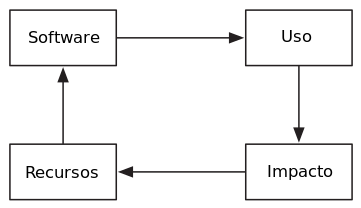
\includegraphics[scale=0.5]{imagens/process-model-scientific-software-dia.png}
  \caption{Um modelo de processo de software na Ciência~\cite{howison2015understanding}}
  \label{process-model-scientific-software}
\end{figure}

A Figura \ref{process-model-scientific-software} apresenta um modelo de
desenvolvimento de software acadêmico, explicitando as relações entre os
elementos \textit{software}, \textit{recursos}, \textit{uso} e
\textit{impactos}, detalhados a seguir.

\subsection{Software acadêmico}

Software acadêmico ({\it academic software}) é todo software usado para
coletar, processar ou analisar resultados de pesquisas com intenção de
publicação na literatura acadêmica (periódicos, revistas, conferências,
monografias, livros ou teses), incluindo desde protótipos escritos pelos
próprios cientistas, a produtos completos desenvolvidos profissionalmente
\cite{allen2017engineering}.

Podem ser projetos de software desenvolvidos num modelo de {\bf Software como
serviço de suporte} ({\it Software as Supporting Service}), sobrevivendo
totalmente à parte do sistema de reputação acadêmica, ou no modelo de {\bf
Software para crédito acadêmico} ({\it Software for academic credit}), estando
seu desenvolvimento intrinsecamente associado ao sistema de reputação acadêmica
\cite{howison2011scientific}.

No segundo caso, Software para crédito acadêmico, a relação com o sistema de
reputação acadêmica pode ainda variar entre motivações distintas resultando em
(1) Software Incidental ({\it Incidental software})
feito puramente para apoiar e facilitar pesquisas,
(2) Prática de software paralela ({\it A parallel software practice})
feito com objetivo de ser utilizado por outros pesquisadores, ou
(3) Um subcampo de software ({\it A Software Subfield}),
onde o próprio software é considerado uma contribuição primária para a Ciência
\cite{howison2011scientific}.

%reputação direta pelo trabalho com o software.
%geralmente publicado em artigo de ferramenta em paralelo aos artigos sobre 
%a pesquisa principal sobre o domínio sendo estudado,

%Garante sua sobreviência independente do sistema de reputação acadêmica,
%geralmente software comercial,
%feito por desenvolvedores de software contratados,
%não costuma receber menção na literatura acadêmica.


  %Software for academic credit
  %\item [Software para crédito acadêmico]

%Está intrinsecamente associado ao sistema de reputação acadêmico,
%tendo como principal incentivo o crédito acadêmico, sendo desenvolvido
%como um Software Incidental ({\it Incidental software})
%feito puramente para apoiar e facilitar a pesquisa,
%como Uma Prática de Software Paralela ({\it A parallel software practice})
%feito com objetivo de ser utilizado por outros pesquisadores,
%geralmente publicado em artigo de ferramenta em paralelo aos artigos sobre 
%a pesquisa principal sobre o domínio sendo estudado,
%como Um Subcampo de Software ({\it A Software Subfield}),
%onde o software é considerado uma contribuição primária para a ciência,
%reputação direta pelo trabalho com o software.

%Incidental software
%typically written by individuals and not made available for
%others to use, at least not in any formal or on-going way.
%
%  %
%  [Uma prática de software paralela]
%        (scientific needed enhanced by publishing 'software papers' alongside domain research)
%
%  %
%  [Um subcampo de software]
%        (reputação direta pelo trabalho do software);
%o segundo sistema de produção que está associado ao crédito acadêmico
%publicações sobre software costuma ser visto como contribuição primária

  %Hybrids
%  \item [Híbridos]
%        licença-dual e 'software work' dentro de grandes colaborações (software como uma contribuição científica direta)
%
%\end{description}

%Software acadêmico também é referenciado na literatura acadêmica como
%{\it research tool} \cite{Portillo12},
%{\it research-originated software} \cite{Kon2011},
%{\it research software} \cite{hettrick2014uk} ou
%{\it scientific software} \cite{segal2008developing}.
%%esses artefatos tem sido estudados dos mais variados pontos
%%de vista, desde de sua qualidade interna, até o impacto que
%%causam no meio científico.

% Proprietary versus public domain licensing of software and research products
% este paper mostra que usar GPL em software traz vantagens e fala dos problemas em nao disponibilizar software academico

%Entre as inúmeras funções desempenhadas pelo software acadêmico em suas
%pesquisas, identificam-se motivações distintas para a sua criação,
%seis modelos de produção de software na ciência que abstraem uma série de
%características sobre como são criados, mantidos e compartilhados,
%estes modelos são caracterizados especialmente pelos incentivos e
%recompensas disponíveis aos seus atores e estão associados a um conjunto de
%práticas de engenharia de software \cite{howison2011scientific}.

\subsection{Recursos}

Os recursos investidos na produção de software acadêmico vêm de diversas
fontes, incluindo ganhos monetários diretos, recursos alocados em projetos, e
colaboração entre laboratórios de pesquisa \cite{howison2015understanding}.
Grande parte dos recursos vem do ``tempo livre'' dos pesquisadores em busca de
soluções para suas pesquisas e perpassa por financiamentos diversos obtidos na
carreira individual do cientista, prêmios recebidos, etc
\cite{howison2015understanding}.

Independente da origem dos recursos, grande parte do desenvolvimento de
software acadêmico é realizado pelos próprios cientistas \cite{hettrick2014uk,
momcheva2015software}.
Esta tendência tem sido interpretada como um reflexo do conhecimento sobre
domínio da pesquisa muitas vezes necessário ao desenvolvedor deste software
\cite{segal2008developing}.

No caso da pesquisa em Engenharia de Software, este conhecimento teórico sobre
o domínio se confunde, muitas vezes, com a própria prática de desenvolvimento.

\subsection{Uso}

% ... software é distribuido, utilizado e dá suporte à ciencia, gerando impacto ...

Metade dos pesquisadores de todas as áreas da Ciência fazem uso intenso de
software acadêmico, desde grupos trabalhando exclusivamente com problemas
computacionais até grupos em laboratórios tradicionais ou em campo
\cite{wilson2014best}.

Este uso é mencionado em suas pesquisas, por meio de citação formal ou informal
\cite{smith2016software}.
Estas menções são parte do sistema econômico de reputação científica e causam
impacto científico direto tanto na publicação quanto no ecossistema de software
acadêmico\cite{katz2014transitive}.

Este impacto direto geralmente justifica o investimentos de novos recursos no
ecossistema, seja para fins de planejamento, como retrospectiva para avaliar
investimentos já realizados ou para promover evolução do software acadêmico
\cite{howison2015understanding}.

\subsection{Impacto científico}

Ao longo da história, a citação formal tem sido utilizada para garantir
autenticidade e autoridade, ao invés de crédito e reconhecimento
\cite{katz2014transitive}.
Na história ocidental, a citação surge no final do século XVI e, no início do
século XVIII surgem o sistema legal por trás do sistema de citações e a lei de
``copyright'' para garantir os direitos dos autores \cite{katz2014transitive}.

Apesar do grande uso para garantir autenticidade e autoridade, o sistema de
citações e a informação sobre a autoria das publicações tem sido realmente
utilizado para avaliações importantes dentro do corpo científico
\cite{katz2014transitive}.
Por exemplo, ``backward citing'' tem sido utilizado para se certificar quem de
fato contribuiiu para um certo avanço ou descoberta, e ``forward citing'' tem
sido usada em casos onde se quer entender como uma idéia foi usada após o seu
surgimento ou publicação \cite{katz2014transitive}.

%Tradicionalmente, um autor cita um artigo anterior adicionando uma referência 
%ao autor, título, local de publicação, etc.

Conhecimento novo é claramente construído a partir do conhecimento passado e o
sistema de citações formais tem promovido avanços significativos
\cite{katz2014transitive}.
No entanto, esse conceito não tem funcionado tão bem para produtos digitais
como o software, que muitas vezes depende de outro software, fragmentos de
código, e algoritmos \cite{katz2014transitive}.

Este debate ocorre há bastante tempo entre as diversas áreas da bibliometria,
cienciometria, altmetria e áreas similares \cite{gouveia2013altmetria}.
Por exemplo, o fator de impacto, proposto na década de 90
\cite{reuters2017history}, apesar de contribuir para a Ciência, por
vezes é utilizado da forma errada e mostra as deficiências de lidar bem com
produtos digitais gerados durante pesquisas \cite{katz2014transitive}.

%%% PAREI AQUI %%%

%%%%%%%%%%%%%%%%%%%%%%%%%%%%%%%%%%%%%%%%%%%%%%%%%%%%%%%%%%%%%%%%%%%%%

%Cita um mapeamento feito sobre estudos que criam ferramentas para apoio a
%revisão sistemática no domínio de SE, 14 estudos foram selecionados, ao final
%apenas 8 tinham proposta de ferramentas, ao final conclui que as ferramentas
%encontradas estão em estado inicial de desenvolvimento \cite{marshall2013tools}.

%Cita um mapeamento sistemático com objetivo de encontrar ferramentas de
%comunicação e coordenação para suporte a times altamente distribuidos
%gograficamente, encontrou 132 ferramentas, para uso em projetos de software
%global. A maioria destas ferramentas foram desenvolvidas em centros de
%pesquisas, e apenas uma pequena porcentagem (18.9\%) foram testados fora do
%seu contexto onde foi desenvolvido \cite{Portillo12}.

%Computer systems research spans sub-disciplines that in-
%clude embedded and real-time systems, compilers, network-
%ing, and operating systems. Our contention is that a number
%of structural factors inhibit quality research. We highlight
%some of the factors we have encountered in our work and ob-
%served in published papers and propose solutions that could
%both increase the productivity of researchers and the quality
%of their output \cite{Vitek2011}.

%Além da aplicação, estes softwares variam também no papel que ocupam em suas
%pesquisas, alguns fazem parte dos resultados da pesquisa, como por exemplo,
%propostas de novos algoritmos ou técnicas de produção, outros são utilizados
%como parte do método de pesquisa, como coleta ou análise de dados, sendo que
%estes papeis não são excludentes.
%
%estes costumam ser citados pelos seus autores como uma das contribuições do
%estudo, seja principal ou secundária, 
%Esses softwares podem, de fato, ser um software de simulação complexo desenvolvido
%e executado em um computador de alto desempenho, mas também pode ser um
%software desenvolvido em um PC para incorporação em instrumentos; para
%manipular, analisar ou visualizar dados; ou para orquestrar fluxos de trabalho.

%e à medida
%que percebe-se que os softwares estão se tornando parte integrante dos
%processos, ferramentas e produção científicas, torna-se necessário e urgente
%discutir o seu desenvolvimento, visibilidade, qualidade e sustentabilidade.

% mostrar os beneficios da ciencia aberta, ciberinfraestrutura, etc
% * (favorecendo a ciencia e tornando a vida mais feliz para todos)

% mostrar os problemas para a ciência como um todo
% * causando problemas para o progresso de ciência, dados perdidos, etc, retrabalho
%   dificuldade de reprodução, etc...

%, não apenas técnica, mas também a
%capacidade de ser encontrado, compartilhado e co-desenvolvido, qualidades
%importantes para a evolução do próprio software, mas também extremamente útil
%para um uso eficiente dos limitados recursos da ciência \cite{howison2013,
%katz2014transitive}.

%contradizendo as boas
%práticas de qualquer projeto experimental, de ter {\it laboratory
%notebooks}\footnote{\url{https://en.wikipedia.org/wiki/Lab_notebook}}, dados
%organizados, passos documentados, e projeto estruturado para reprodutibilidade.

%softwares acadêmicos, assim
%como qualquer outro aparato experimental, são tão importantes para a ciência
%quanto são os telescópios ou tubos de ensaio \cite{wilson2014best}.

%Cientistas gastam mais tempo hoje utilizando e desenvolvendo softwares do que
%gastavam no passado.

%Software is a critical part of modern research and yet there is little support across the
%scholarly ecosystem for its acknowledgement and citation. Inspired by the activities
%of the FORCE11 working group focused on data citation, this document
%summarizes the recommendations of the FORCE11 Software Citation Working
%Group and its activities between June 2015 and April 2016. Based on a review of
%existing community practices, the goal of the working group was to produce a
%consolidated set of citation principles that may encourage broad adoption of a
%consistent policy for software citation across disciplines and venues. Our work is
%presented here as a set of software citation principles, a discussion of the motivations
%for developing the principles, reviews of existing community practice, and a
%discussion of the requirements these principles would place upon different
%stakeholders. Working examples and possible technical solutions for how these
%principles can be implemented will be discussed in a separate paper.
%\cite{smith2016software}

%Improving academic software engineering projects: A comparative study of academic and industry projects
%(compara as praticas de desenvolvimento da industria e academia e sugere melhorias, 1998!)
%https://link.springer.com/article/10.1023%2FA%3A1018925902814?LI=true

% papel pesquisador no ecossistema de soft academico
%
%Essas preocupações gerais sugerem um conjunto de questões específicas, com foco
%em padrões globais e padrões emergentes dentro do ecossistema, incluindo: Quais
%recursos foram destinados à produção de software? Quantos usuários ou
%comunidades de usuários têm projetos? Quais são os impactos científicos desse
%uso? Os números de usuários crescem? Os projetos possuem recursos e habilidades
%suficientes para gerenciar seu crescimento? Quais projetos possuem
%funcionalidades sobrepostas? Há quanto tempo os pedaços de software e projetos
%persistem? Nós desconectamos as comunidades de usuários e desenvolvedores? São
%componentes específicos, ou camadas de componentes, faltam? Que código
%geralmente é usado em conjunto; são os projetos e as pessoas que produzem esses
%componentes se comunicando adequadamente? Como podemos sustentar o software
%crítico?
%
%Aqui há uma clara tensão entre um desejo de flexibilidade e liberdade, ligado
%às expectativas de inovação científica e desejos de estruturas de autoridade e
%controle de coordenação. As questões de influência incluem: como os programas
%de financiamento e quais os requisitos em suas chamadas, resultaram em software
%amplamente utilizado e impacto científico substancial? Quais são as
%características dos campos que alcançaram maior coalescência? Quais jornais e
%conferências têm políticas exemplares? Como o trabalho de software é visto
%dentro das práticas de contratação e avaliação, como os casos de posse?
%
%\cite{howison2015understanding}

%Ao longo da história, a citação formal foi para autenticação e autoridade, em
%vez de de crédito e reconhecimento ou atribuição. A  científico citação na
%história ocidental aparece no final dos anos 1500. No início dos anos 1700, a
%citação também aparece no sistema legal como método de compreensão dos
%precedentes \cite{katz2014transitive}.

%A ideia de direitos autorais como reconhecendo aos direitos dos seus autores
%também surge nesse tempo, 1710, talvez devido a uma lenta tendência social
%societária de reconhecer a propriedade intelectual, uma idéia que parece ter se
%desenvolvido ao lado da imprensa]. Observe que a autoria de papers é realmente
%usado para notar os autores reais do artigo quanto para notar os contribuidores
%do projeto.
%Para muitos desses, o
%identificador que deve ser citado - um "nome" que se refere a um produto único
%não é claro.

%Additionally, if a cited library depends
%on another library, the contribution of this second library
%is not captured. Citation of a dataset should perhaps give
%credit to the people who gathered the data, as well as
%those who curated it, but the paper author may not know
%or be able to find these details.

%Mas independente de como seja calculado o impacto científico de uma determinada
%pesquisa o impacto causado se reverte potencialmente em mais recursos que
%poderão ser reinvestidos no próprio ecossistema onde o software está inserido.

%Science Code Manifesto \cite{barnes2013science}.
%Foco em código fonte escrito especificamente para processar dados de
%publicações, afirma que ``todo código fonte escrito especificamente para
%processar dados de uma publicação deve estar disponível para os revisores e
%leitores do paper''.

%Sustentabilidade é um conceito guarda chuva composto de múltiplas dimensões, em
%sua dimensão técnica, chamada sustentabilidade técnica, temos a preocupação com
%a longevidade da informação, dos sistemas, e infraestrutura, e sua adequada
%evolução frente as condições do ambiente em constante mudança.

%citações formais facilitam e promovem o avanço
%da ciência, mesmo diante da falta de um padrão para citar artefatos digitais
%\cite{allen2014credit}.

%Um estudo recente com 90 artigos de diversas áreas da biologia, selecionados
%aleatoriamente entre publicações usando softwares como método, mostrou que
%apenas 59 mencionavam o uso de softwares de alguma forma, os demais 31 artigos,
%apesar de usar software acadêmico, não mencionavam nada a respeito
%\cite{howison2016software}, apenas entre 31\% e 43\% das menções aos softwares
%acadêmicos envolvem citação formal.

%Não existe ainda amadurecimento suficiente sobre como citar softwares e
%outros artefatos digitais em pesquisas científicas, não temos um padrão de como fazê-lo,
%cada autor cita à sua maneira, muitas vezes ao longo do texto, outras em seções
%específicas sobre a implementação do software, nem semprem informam onde
%encontrar uma cópia do software, ou ainda nem sobre o modelo em que o software
%é distribuído, ou se é de alguma forma distribuído ao público.

%Entre os softwares acadêmicos desenvolvidos por cientistas como apoio em suas
%pesquisas, não é raro que pesquisadores deixem de disponibilizar estes artefatos,
%assim como outros desdobramentos da pesquisa, como dados e outros. Ou ainda,
%mesmo disponibilizando tais artefatos em locais de público acesso, com o tempo,
%tais locais se tornam indisponíveis inviabilizando a obtenção de tais
%artefatos.

%A comunidade tem refletido sobre os problemas relacionados ao
%desenvolvimento, promoção e sustentabilidade desses softwares, e o
%impacto que tais problemas causam no meio científico \cite{allen2017engineering}.

%, e faz
%surgir questionamentos sobre sua qualidade, não apenas técnica, mas também a
%capacidade de ser encontrado, compartilhado e co-desenvolvido, qualidades
%importantes para a evolução do próprio software, mas também extremamente úteis
%para o uso eficiente dos limitados recursos da ciência \cite{howison2013,
%katz2014transitive}.

%, o ecossistema de software acadêmico por
%exemplo possui a particularidade de estar inserido no sistema de reputação
%científica de alguma forma.

%os atores recebem mais (ou melhores) benefícios com o crescimento
%do ecossistema, o ecossistema oferece cada vez mais (ou melhores) benefícios
%com as atividades dos seus atores, resultando numa relação de benefício
%mútuo.

%e pelo seu sistema de crédito acadêmico.

% (5) Tools in mining software repositories \cite{chaturvedi2013tools}
% Faz uma revisão dos papers submetidos ao MSR desde 2007 até 2013 (?) e
% identifica data sets, ferramentas e técnicas utilizadas pelos autores, mais
% da metade dos papers usam ou criam ferramentas, categoriza as ferramentas em
% ferramentas novas, ferramentas tradicionais, protótipos e scripts para
% mineração de dados

%que podem ser adotadas por outros cientistas,
%especialmente em outros domínios. 

%preocupam-se com o impacto cientifico tanto em termos de numero
%quando de tipos de usuários que seu software atinge, 

%a partir da evolução deste software ou a partir da produção de novo software.


\section{Ecossistema de software acadêmico de análise estática} \label{analise-estatica}

Ao falarmos sobre ecossistema de software acadêmico estamos nos referindo a
qualquer software, de qualquer domínio de aplicação, que tenha sido utilizado
ou produzido durante trabalhos de pesquisa com intuito de publicação na
literatura acadêmica.
%REVER - intuito de apoiar pesquisa que será eventualmente divulgada por meio da  publicação de resultados.

O ecossistema de software acadêmico de análise estática é um recorte deste
conjunto, a princípio, com as mesmas características, atores e modelo de
funcionamento, mas logicamente podendo de apresentar particularidades trazidas
pela natureza do domínio de análise estática e suas ferramentas, soluções e
algoritmos.

\subsection{Análise estática}

A análise estática de código fonte é o primeiro passo para coletar informações
necessárias em diversas atividades de verificação, medição e melhoria da
qualidade de produtos de software \cite{cruz2009code, kirkov2010source}. Ela é
realizada com base no código fonte de um programa ou sistema de software, e a
partir daí descobre problemas e propriedades de sua qualidade estrutural
\cite{chess2007secure}.

Ferramentas de análise estática estão disponíveis há décadas, em especial,
para programadores. A ferramenta Lint \cite{johnson1978lint}, considerada a
primeira ferramenta de análise estática \cite{gosain2015static}, foi criada para
examinar programas escritos em linguagem C e aplicar regras de tipagem mais
estritas do que as regras dos próprios compiladores da linguagem.

Análise estática de código fonte tem como objetivo prover
informações acerca de um programa a partir do seu código fonte sem
necessidade de execução, e sem requerer qualquer outro artefato do programa
além do próprio código.

É um ramo que possui muitas das suas abordagens em comum com os estudos da
área de análise de programas ({\it program analysis}), especialmente na área de
compiladores, onde atua especialmente nas primeiras etapas do processo de compilação.

A análise estática de código fonte é considerada uma atividade meio com
objetivo de suportar uma variedade de tarefas comuns da engenharia de
software; muitas dessas tarefas são substancialmente úteis em atividades de
manutenção. Binkley~\citeonline{binkley2007source} define uma lista dessas
atividades, incluindo:

\begin{multicols}{2}
  \begin{itemize}
    \item Análise de performance
    \item Compreensão de programas
    \item Desenvolvimento baseado em modelos
    \item Detecção de clones
    \item Evolução de software
    \item Garantia de qualidade
    \item Localizaçao de falhas
    \item Manutenção de software
    \item Recuperação arquitetural
    \item Testes
  \end{itemize}
\end{multicols}

Seja em qual atividade for, a análise estática possui importância,
pois ao ser capaz de extrair informações diretamente do
código fonte de um programa, pode auxiliar a responder perguntas necessárias
para as diversas atividades de desenvolvimento e evolução de software. Essa
importância se torna ainda mais aparente diante da ``lei'' da tendência para
execução \cite{harman2010why} que indica que todos os tipos de notação tem a
tendência de se tornar executáveis.

% \subsection{Usos da análise estática de código fonte} \label{usos}

A análise de programas trata, de modo geral, da descoberta de problemas e
fatos sobre programas. Tal análise pode ser realizada sem a necessidade de executar o
programa (análise estática) ou com informações provenientes de sua execução
(análise dinâmica).

A ideia de que programas de computador podem ser utilizados para analisar
código fonte de outros programas tem uma história de mais de 40 anos.  O
programa PFORT \cite{ryder1974pfort} foi projetado para localizar potenciais
problemas na portabilidade de código Fortran; em função da diversidade de
dialetos de Fortran, uma compilação sem erros não indicava que o programa
estava correto segundo os padrões da linguagem \cite{wichmann1995industrial}.

Desde então, ferramentas de análise estática de código fonte têm surgido para
os mais diversos fins -- muitas delas a partir das pesquisas e
desenvolvimentos da área de compiladores.  O {\it parser} utilizado nessas
ferramentas têm funcionalidades análogas aos analisadores usados em
compiladores \cite{anderson2008the}.

O uso de tais ferramentas tem se tornado mais comum no ciclo de desenvolvimento de
software, sendo aplicadas em atividades distintas.
O campo de aplicação destas ferramentas é bastante variado, cobrindo diferentes
objetivos.

\subsection{Software de análise estática}

A variedade de aplicação e a constante evolução da área de análise estática, 
tanto na indústria quando na academia, resulta em  estudos teóricos e práticos, novas ferramentas, modelos e
algoritmos de análise estática. Ferramentas de análise estática têm sido
continuamente desenvolvidas e seu uso se tornado comum no ciclo de desenvolvimento de
software.

Mas apesar da rápida e constante evolução da área, ainda há carência de estudos
avaliando estas ferramentas \cite{li2010comparative}, mesmo com os avanços e com
ferramentas de sucesso, o desenvolvimento de análise estática ainda é conhecido
por ser um processo doloroso \cite{toman2017taming}.

A eficiência, confiabilidade e precisão dessas ferramentas têm sido avaliadas e
alguns estudos mostram inconsistência entre ferramentas diferentes.
Um estudo que comparou duas ferramentas de análise estática para cálculo de métricas,
revelou significantes evidências sobre a inconsistencia entre valores de métricas,
grande diferença nos valores, e discutiu quais problemas e questões levam a estas
diferenças \cite{alemerien2013experimental}.

Análise estática é a técnica mais amplamente utilizada para análise
automatizada de programas devido a sua eficiência, boa cobertura e automação.
Estudos mostram que analise estática tem grande adoção em projetos de software
livre \cite{beller2016analyzing}.
Entretanto,tecnicas de analise estatica amplamente adotadas na comunidade de software,
por exemplo, para localização de bugs e verificação de programas 
ainda sofrem de alto indica de falso-positivos \cite{gosain2015static}.

A crescente atenção que as técnicas de análise estática de código tem
recebido em pesquisas não necessariamente influencia em sua adoção na indústria,
identificando um gap entre pesquisa e indústria \cite{ilyas2016static}.

\subsection{Software acadêmico de análise estática}

Em Ciência da Computação, particularmente em Engenharia de Software, tem-se
notado um aumento constante no número de novos softwares acadêmicos \cite{allen2017engineering},
especialmente em estudos de análise estática, 
uma área com uma longa e respeitável tradição em
pesquisas sobre a criação de novas ferramentas, métodos e algoritmos.

%Na indústria também a adoção de software de análise estática é crescente...

O software acadêmico de análise estática está inserido no contexto similar
a qualquer outro software acadêmico, e o seu ecossistema possui as mesmas
características do ecossistema de software acadêmico, inserido na economia
de reputação científica, Figura \ref{scientific-reputation-diagram} apresenta
o relacionamento entre a prática e pesquisa de software acadêmico.

\begin{figure}[h]
  \center
  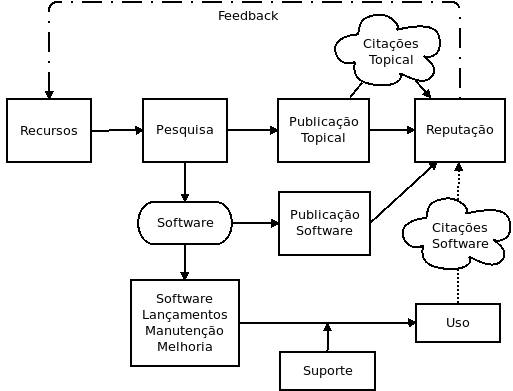
\includegraphics[scale=0.5]{imagens/scientific-reputation-diagram.png}
  \caption{A depiction of the reputation incentives in a mixed science and software academic practice \cite{howison2011scientific}}
  \label{scientific-reputation-diagram}
\end{figure}

%ecossistema de software acadêmico está inserido num contexto de competição

Diferentemente de outras tecnologias, software pode ser copiado e distriduído
essencialmente sem custo, abrindo portas sem precedentes em nível para
compartilhamento e inovação colaborativa \cite{howison2011scientific}, no
entando, estar em algum ponto no contexto de competição da economia de
reputação científica, em alguns pontos, como no mecanismo de crédito acadêmico
às produções ser potencialmente problemático para a colaboração e manutenção
\cite{howison2011scientific}.

No entanto tem se percebido que o ecossistema de software acadêmico tem perdido
oportunidade de colaboração visto que estão inseridos neste contexto ....
competição, muitos softwares utilizados em pesquisas não são mencionados pelos
seus autores causando impacto negativo em sua visibilidade, reconhecimento e
consequentemente ...  \cite{howison2016software}. Esta reflexão tem mostrado,
por exemplo, que muitos estudos em engenharia de software sofrem de
dificuldades de repetição \cite{tang2016worthiness}, e apontam problemas específicos
relacionados à manutenabilidade e a sustentabilidade técnica dos softwares
acadêmicos.

Este cenário, além de desacelerar o progresso geral da Ciência gerando
retrabalho, faz surgir questionamentos sobre as conclusões dessas pesquisas,
especialmente quando grande parte dos pesquisadores não sabem o quão confiável
seus softwares são. Junto com estas questões estão as questões de como
influenciar o ecossistema, incluindo questões de pontos de inflexão que levam
ao uso coalescente, bem como a intervenções políticas diretas incentivando o
uso de componentes específicos.

%%%%%%%%%%%%%%%%%%%%%%%%%%%%%%%%%%%%%%%%%%%%%%%%%%%%%%%%%%%%%%

%While some of these seem relatively unproblematic, such as commercial
%production in fields with immediately valuable applications, others appear
%problematic. In particular we highlighted the potentially pernicious
%implications of the academic credit production system for collaboration and
%maintenance 

%Adicionalmente as relacões entre os atores do ecosistema como um todo
%são de mútuo interesse (mutualismo):

%O relacionamento entre os atores em um ecossistema de software, por outro lado,
%são caracterizados pela alto espectro de relacionamentos simbioticos.

%Dependendo dos atores e suas atividades, dois atores podem ter benefícios
%mútuos (mutualismo), estar em competição direta (competition/antagonism),
%estarem não afetados (neutralism) ou um não afetado enquanto o outro é
%beneficiado (amensalism) ou prejudicado (parasitism) por seu relacionamento

%em pesquisas sobre análise de código, ferramentas de analise estatica tem
%recebido significante mais atencao que outras tecnicas, tecnicas com formal e
%bem definidos processos recebem mais atencao de pesquisa e escrutinio porque
%estudos irao avaliar seu processo e elementos, entretanto, isto nao
%necessariamente significa que tecnica é melhor; The survey concluded that 1)
%the adoption of static code analysis techniques in the industry is influenced
%by the software life cycle model, while software product type and company size
%doesn’t have an influence. 2) The amount of attention a static code analysis
%technique has received in research doesn’t necessarily influence its adoption
%in industry indicating a gap between research and industry 3) company size,
%product type, and life cycle model do influence professionals perception on
%benefits/limitations.  \cite{ilyas2016static}

\section{Sustentabilidade de software acadêmico}

O desenvolvimento de software sustentável tem sido identificado como um desafio
chave no campo da Ciência e da Engenharia Computacional, se sustentabilidade
não for levada em consideração em projetos de software, não importa qual o
domínio ou qual o propósito do software, perde-se a oportunidade de causar
mudanças positivas no planeta e na sociedade \cite{becker2014karlskrona}.

Sustentabilidade de software apesar de ser um conceito complexo e com mútiplas dimensões,
levando a debates profundos, possui um conceito geral bastante simples: refere-se à
capacidade de perdurar e de continuar sendo suportado ao longo do tempo, o que 
implica nas qualidades de longevidade e manunenabilidade do software
\cite{venters2014software}.

%Sustentabilidade de software tem sido um tema de intenso debate e inúmeras definições,
%frameworks, modelos, propostas de tornar sustentabilidade como um requerimento
%não-funcional de software, no entando em todos os em resumo uma conclusão tem sido
%geral e central, entre os frameworks, o contexto onde o software está inserido influencia na medição
%de sustentaabilidade \cite{venters2014software}. No entando, uma definição
%comum e compartilhada ainda não é realidade, não existe ainda uma definição
%clara do que significa sustentabilidade de software, e isto não pode ser
%subestimado. Entretando, esta falta de concenso, junto ao fato de que uma
%visão comum entre as propostas de frameworks para sustentabilidade é de que
%a definição e medição está intimamente relacionada ao contexto, ou domínio do
%problema \cite{venters2014software}, dessa forma uma boa estratégia de colaborar com esta grande figura é
%definir sustentabilidade em recortes distintos, como, sustentabildiade de
%software acadêmico de análise estática, por exemplo.

Software sustentável é aquele que continua a estar disponível no futuro, em
novas plataformas, atendendo continuamente às novas necessidades do ambiente
através de uma adequada evolução frente as condições em constante mudança
\cite{allen2017engineering}. Este conceito, no entando, ao ser aplicado ao
contexto de software acadêmico e artefatos digitais, mostra-nos um cenário
bastante preocupante, uma vez que, estudos recentes mostram que há uma tendêcia
ao decaimento de URLs ao longo do tempo, em publicações com produção de
artefatos digitais disponibilizados nestes endereços tem uma tendência a
tornarem-se indisponíveis ao longo dos anos \cite{wren2017use}.

Isto tem motivado iniciativas de tornar estes artefatos duráveis e disponíveis,
visando especialmente garantir a longevidade dos artefatos e proporcionar que
um segundo pesquisador receba todos os benefícios do trabalho duro do primeiro
pesquisador \cite{king1995replication},
o {\it Journal of the American Statistical Association (JASA)}, por
exemplo, tem insistido na necessiade de estar disponíveis código e dados ao
menos durante a revisão dos manuscritos \cite{baker2016scientists}, agências de
financiamento, como o {\it US National Science Foundation}, estão começando a
reconhecer produtos de pesquisa, como software, assim como fazem com as
publicações, tornando o software produzido em pesquisas cidadão de primeira
classe na Ciência \cite{allen2017engineering}.

Isto garante longevidade mas não implica em boa manutenibilidade, uma qualidade especialmente
importante aos projetos de software acadêmico, visto que sua qualidade tem sido questionada, onde a maioria dos cientistas autores
de software não sabe o quão confiável seu software é
\cite{merali2010computational}, muitos dos projetos de software acadêmico estão
em estado inicial de desenvolvimento \cite{marshall2013tools}, poucos foram
testados fora do contexto onde foram desenvolvidos \cite{portillo2012tools}.

\subsection{Problemas}

Não é difícil perceber que o ecossistema de software acadêmico sofre graves
problemas, percepção bastante similar ao fenômeno chamado de  desordem
caótica disfuncional ({\it ``dysfunctional chaotic churn''}), caracterizado
por:

\begin{quote}
Existência de muitos projetos, com poucos usuários, com
ciclos de vida curtos, que terminam em paralelo ao financiamento inicial,
comunidades desconectadas e paralelas, incompatibilidades entre projetos, e
tentativas aparentemente não coordenadas de ``reiniciar'' tudo ({\it re-boots})
\cite{howison2015understanding}.
\end{quote}

Este problema, apesar de ser apenas uma percepção, coincide com inúmeras
evidências a respeito de problemas com o desenvolvimento, reconhecimento e
sustentabilidade de software acadêmico \cite{allen2017engineering}.

%sabe-se que parte dos problemas são realmente fato, por exemplo,
%o {\it Dagstuhl Perspective Workshop}, evento organizado por um grupo de
%pesquisadores sêniores de renome internacional, realizado anualmente na
%universidade de Dagstuhl\footnote{\url{http://www.dagstuhl.de}} com o objetivo
%refletir sobre o estado da ciência da computação explorando tópicos novos e
%emergentes, em sua mais recente edição o workshop debateu sobre software

\subsubsection{Desenvolvimento}

O desenvolvimento de software acadêmico exige, muitas vezes, conhecimento
específico sobre o domínio do estudo sendo realizado,
por exemplo, entender como o DNA genômico
se transforma em cristais de proteína, ou estar familiarizado com os meandros
da dinâmica dos fluidos, ou saber como resolver 20 equações diferenciais
parciais simultâneas \cite{segal2008developing}.

Isto explica a grande participação dos cientistas no desenvolvimento de
software acadêmico, estudos tem mostrado que no reino unido entre todas as
áreas da ciência 56\% dos cientistas estão envolvidos no desenvolvimento de
software acadêmico \cite{hettrick2014uk}, outros estudos em grupos específicos mostram números ainda
maiores, na astronomia, por exemplo, 90\% dos cientistas desenvolvem software
acadêmico \cite{momcheva2015software}.

No entanto, a maior parte dos cientistas nunca tiveram treinamento algum sobre como escrever
software de forma eficiente, muitos não testam ou documentam os seus projetos de
software, faltam práticas básicas de desenvolvimento, como escrever código
legível, revisão de código, controle de versão, testes unitários, entre outros
\cite{wilson2017good}.

Isto tem ocasionado sérios erros computacionais em conclusões centrais da
literatura acadêmica, gerando retrabalho para retratar tais erros nas mais
diversas áreas da ciência \cite{merali2010computational}.
Dados são perdidos, análises levam mais tempo que o necessário e os
pesquisadores não conseguem a eficiência que poderiam ter ao trabalhar com
software acadêmicos \cite{wilson2017good}.
Causando um impacto negativo na visibilidade do software acadêmico e na
capacidade de ser encontrado e compartilhado \cite{howison2013incentives,
katz2014transitive}.

\subsubsection{Reconhecimento}

% visibilidade

Apesar do crescimento no uso de software e na consequente dependência entre
cientistas de todos os campos, tornando o software acadêmico parte integral da
prática científica, apesar do apelo da comunidade científica para que o
software acadêmico seja tratado como cidadão de primeira classe, estudos tem
mostrado que muitas pesquisas não mencionam sequer o uso de software acadêmico
em suas publicações mesmo tendo feito uso de tais artefatos
\cite{momcheva2015software} \cite{howison2016software}.

Isto tem prejudicado a visibilidade do software acadêmico causando impacto
negativo em seu ecossistema, um software invisível é frequentemente excluído de
revisões por pares, uma atividade que costuma contribuir para a qualidade geral
do trabalho publicado, além disso, o
impacto negativo na visibilidade do software acadêmico faz surgir uma
série de questionamentos sobre a sua qualidade e também sobre a
capacidade de ser encontrado, compartilhado e co-desenvolvido
\cite{howison2013incentives, katz2014transitive} \cite{howison2016software}.

Apesar de nem sempre ser possível, ou viável, ter tudo dentro de padrões
estritos, é preciso estar consciente das boas práticas ao produzir e utilizar
software acadêmico, tanto para melhorar a própria abordagem quanto para
revisar outros trabalhos \cite{wilson2014best}. Um software acadêmico em bom
funcionamento devem atingir não apenas os objetivos de entendimento e
transparencia, mas também os objetivos voltados para replicação
\cite{stodden2010reproducible}, seja logo após sua publicação, seja daqui a 10 ou 50 anos.

\subsubsection{Manutenibilidade}

% falar de manutenibilidade como um eixo dentro de sustentabilidade técnica

Manutenibilidade é uma característica de qualidade que indica o quão fácil é
realizar atividades de evolução e manutenção em software
\cite{kumar2012survey}, um aspecto importante aos pesquisadores interessados em
adaptar software acadêmico, algo muitas vezes necessário ao reproduzir
pesquisas anteriores \cite{peng2011reproducible}.

Estudos tem mostrado que grande parte das ferramentas de software criadas na
academia estão em estado inicial de desenvolvimento \cite{marshall2013tools} e
que apenas uma pequena porcentagem são testados fora do contexto onde foi
desenvolvido \cite{portillo2012tools}.

%A adoção e uso de software acadêmico está relacionado também à sua qualidade,
%portanto é importante medir e coletar sua qualidade de alguma forma, qualidade
%é um vasto assunto, um dos problemas comuns enfrentado pelos pesquisadores que
%desenvolvem tais projetos de software é a manutenibilidade \cite{prlic2012ten}.

A adoção e uso de software acadêmico está relacionado também à sua qualidade,
portanto é importante medir e coletar sua qualidade de alguma forma,
manutenibilidade apesar de ser um atributo de qualidade de software
inerentemente externa, pode ser medida através de
características de qualidade interna \cite{hashim1996software,
dagpinar2003predicting}, uma vez que grande parte dos engenheiros de software
assumem que uma boa estrutura interna resulta em boa qualidade externa
\cite{fenton2014software}.

No entanto é importante compreender os projetos de software acadêmico também em
termos de evolução e ciclo de vida, algo que pode influenciar enormemente as
medidas de qualidade medidas através de atributos internos do software, como
métricas de código fonte, por exemplo. 

%Iniciativas desta natureza resolvem o problema de disponibilidade destes
%artefatos mas ainda não garantem adequada evolução frente a contínua mudança
%do ambiente, apesar de sustentabilidade não implicar diretamente em qualidade,

%Tanto a ciência quanto a
%engenharia dependem de resultados incrementais para sua evolução. No terceiro
%compromisso, relacionado ao conceito {\it desenvolvimento}, o Dagstuhl
%Manifesto enfatiza a necessidade de medir a qualidade e a sustentabilidade dos
%softwares científicos, tanto a priori quanto a posteriori.

%Um estudo sobre ecossistema de software acadêmico percebeu através dos relatos
%de grande parte dos colaboradores participantes do estudo que os projetos de software
%acadêmicos desenvolvidos na própria academia 

%Olhar melhor os atributos de qualidade no artigo de Venters:
% https://openresearchsoftware.metajnl.com/articles/10.5334/jors.ao/
% We propose that software sustainability should be considered in a similar manner to the concept of dependability[16]; 
% a measure of a system’s availability, integrity, maintainability, reliability, and safety 
% where the attributes of dependability are defined as:
% Availability: readiness for correct service;
% Integrity: the absence of improper system alteration;
% Maintainability: undergo modifications and repairs;
% Reliability: continuity of correct service;
% Safety: the absence of catastrophic consequences on the user(s) and the environment.

%\begin{comment}
%
%We propose that software sustainability can be defined as ‘a measure of a systems extensibility, interoperability, maintainability, portability, reusability, scalability, and usability’ where the attributes are defined as:
%Extensibility: a measure of the software’s ability to be extended and the level of effort required to implement the extension;
%Interoperability: the effort required to couple software systems together.
%Maintainability: the effort required to locate and fix an error in operational software;
%Portability: the effort required to port software from one hardware platform or software environment to another;
%Reusability: the extent to which software can be reused in other applications;
%Scalability: the extent to which software can accommodate horizontal or vertical growth.
%Usability: the extent to which a product can be used by specified users to achieve specified goals with effectiveness, efficiency, and satisfaction in a specified context of use.
%If we accept that the concept of sustainability goes beyond the software artifact itself then other quality attributes such as efficiency may be appropriate candidates:
%Efficiency: the amount of computing resources and code required to execute a function.
%
%\end{comment}

\section{Ciclo de vida de software}
\label{sec:ciclo}

Engenheiros de software têm tradicionalmente considerado qualquer trabalho após
o primeiro lançamento de um software simplesmente como manutenção. Alguns
pesquisadores no entanto têm dividido este trabalho em atividades distintas, incluindo
adaptação, prevenção, correção, entre outras, mas sempre considerando manutenção
basicamente uniforme ao longo do tempo \cite{rajlich2000staged}.

Entretanto, alguns estudos têm demonstrado que esta visão, onde manutenção
ocupa um papel basicamente uniforme ao longo do tempo, não explica muito bem o
desenvolvimento de software na maior parte dos cenários e uma das abordagens
para explicar o fenômeno tem colocado a atividade de manutenção distribuída ao
longo do ciclo de vida do software \cite{rajlich2000staged}.

Este modelo de evolução do software em estágios, no entanto, foi avaliado e adaptado
ao contexto de software livre \cite{capiluppi2007adapting} e diante das
semelhanças com o software acadêmico, este modelo adaptado ao software livre serve ao propósito de ser
utilizado para
avaliar a evolução do software acadêmico. A Figura \ref{staged-model-foss-cycle}
apresenta o modelo de evolução adaptado ao software livre, adotado
neste estudo como aplicável também ao software acadêmico.

\begin{figure}[h]
  \center
  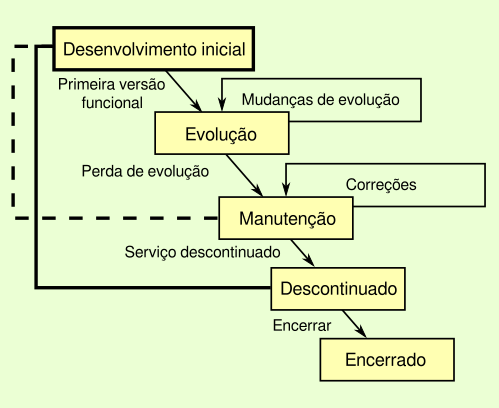
\includegraphics[scale=0.6]{imagens/staged-model-foss-cycle.png}
  \caption{O modelo de evolução {\it staged model} adaptado a software livre \cite{capiluppi2007adapting}.}
  \label{staged-model-foss-cycle}
\end{figure}

A primeira diferença observada é em relação a fase {\it Desenvolvimento inicial},
dependendo da definição de ``fase inicial'' muitos projetos de software livre
podem nunca ter saído desta fase, assim é também para o software acadêmico. Em respeito aos lançamentos,
em sistemas comerciais tradicionais eles devem ser completos, rodando e autorizado
pela empresa detentora, enquanto no mundo do software livre é comum
permitir acesso público ao código em repositórios de código fonte, seguindo
um modelo de ``versão permanente''.

A segunda diferença é relacionada à possibilidade de laços entre
as fases {\it Evolução} e {\it Manutenção}. Muitos projetos de software livre
possuem fases de congelamento na adição de novas funcionalidades ({\it freeze})
enquanto permanece numa fase de {\it Manutenção} até o descongelamento, voltando
a {\it Evolução}.

A terceira diferença está na comunidade de software livre,
novos times de desenvolvimento são formados ao longo do tempo
com a saída de desenvolvedores antigos e a entrada de novos.
E projetos em fase {\it Descontinuado} podem experimentar um renascimento
retornando ao período de {\it Evolução}.

Apesar das diferenças, os autores \citeonline{capiluppi2007adapting} demonstram em experimentos e
revisão de literatura que o modelo adaptado pode ser utilizado para
compreender evolução de software livre, e diante as similaridades entre software livre
e software acadêmico, este modelo poderá, consequentemente, ser também
utilizado para compreender a evolução e ciclo de vida do software acadêmico.

